\section{Capsules}\label{sec:capsules}

\subsection{What a capsule is}

A capsule is a statically linked position-independent ELF built offline for the target \code{x86\_64-nonos-user}, plus three files: a \nonos{} ID certificate, a binary manifest and an attestation trailer. Authors do not write manifests. They set \code{CAPSULE\_*} variables in a \code{Capsule.mk}, and the build produces the manifest.\srcs{docs/userland/README.md}{docs/userland/manifests-and-capabilities.md} There are 152 \code{Capsule.mk} files in the tree. Each names the capsule's service, its endpoints and its capability word, and the same facts appear again in the kernel's own copy, which a script holds to the manifest.\src{scripts/check_mirror_caps.py}

\subsection{The manifest}

The manifest is schema version 3 and big-endian. In wire order it carries the schema version; a certificate id, the BLAKE3 hash of the \nonos{} ID certificate; a namespace of 1 to 96 bytes; a version; the target triple; a payload hash, the BLAKE3 hash of the whole ELF; the required capability word; the optional word, which must not overlap the required one; up to 16 endpoints; and one to four signatures.\srcs{src/security/capsule_manifest/schema/constants.rs:17-25}{src/security/capsule_manifest/decode/mod.rs:25-47} The publisher signs every byte before the signature count. Algorithm 1 is Ed25519 with 64-byte signatures and algorithm 3 is ML-DSA-65 with 3309-byte signatures.\src{src/crypto/asymmetric/alg_id/lengths.rs:19-26}

\subsection{Admission}

Figure~\ref{fig:admit} shows admission at spawn. The certificate must verify under the trust anchor with both algorithms, must not be stale or revoked, and bounds what the publisher may request through a capability ceiling and namespace globs. The manifest must then verify under the publisher's keys with both algorithms, and its payload hash must equal the BLAKE3 of the ELF being loaded. Finally the STARK gate checks the capsule's slot under the compiled-in policy root, with the manifest's required capability word as part of the statement. A capsule enrolled with one set of rights therefore cannot open with another.\src{src/kernel_core/process_spawn/capsule_spawn/runner/preflight.rs:36-76} Only after all three checks does the kernel create the process, install the word and record the measurement in the attestation registry.

\begin{figure}[t]
\centering
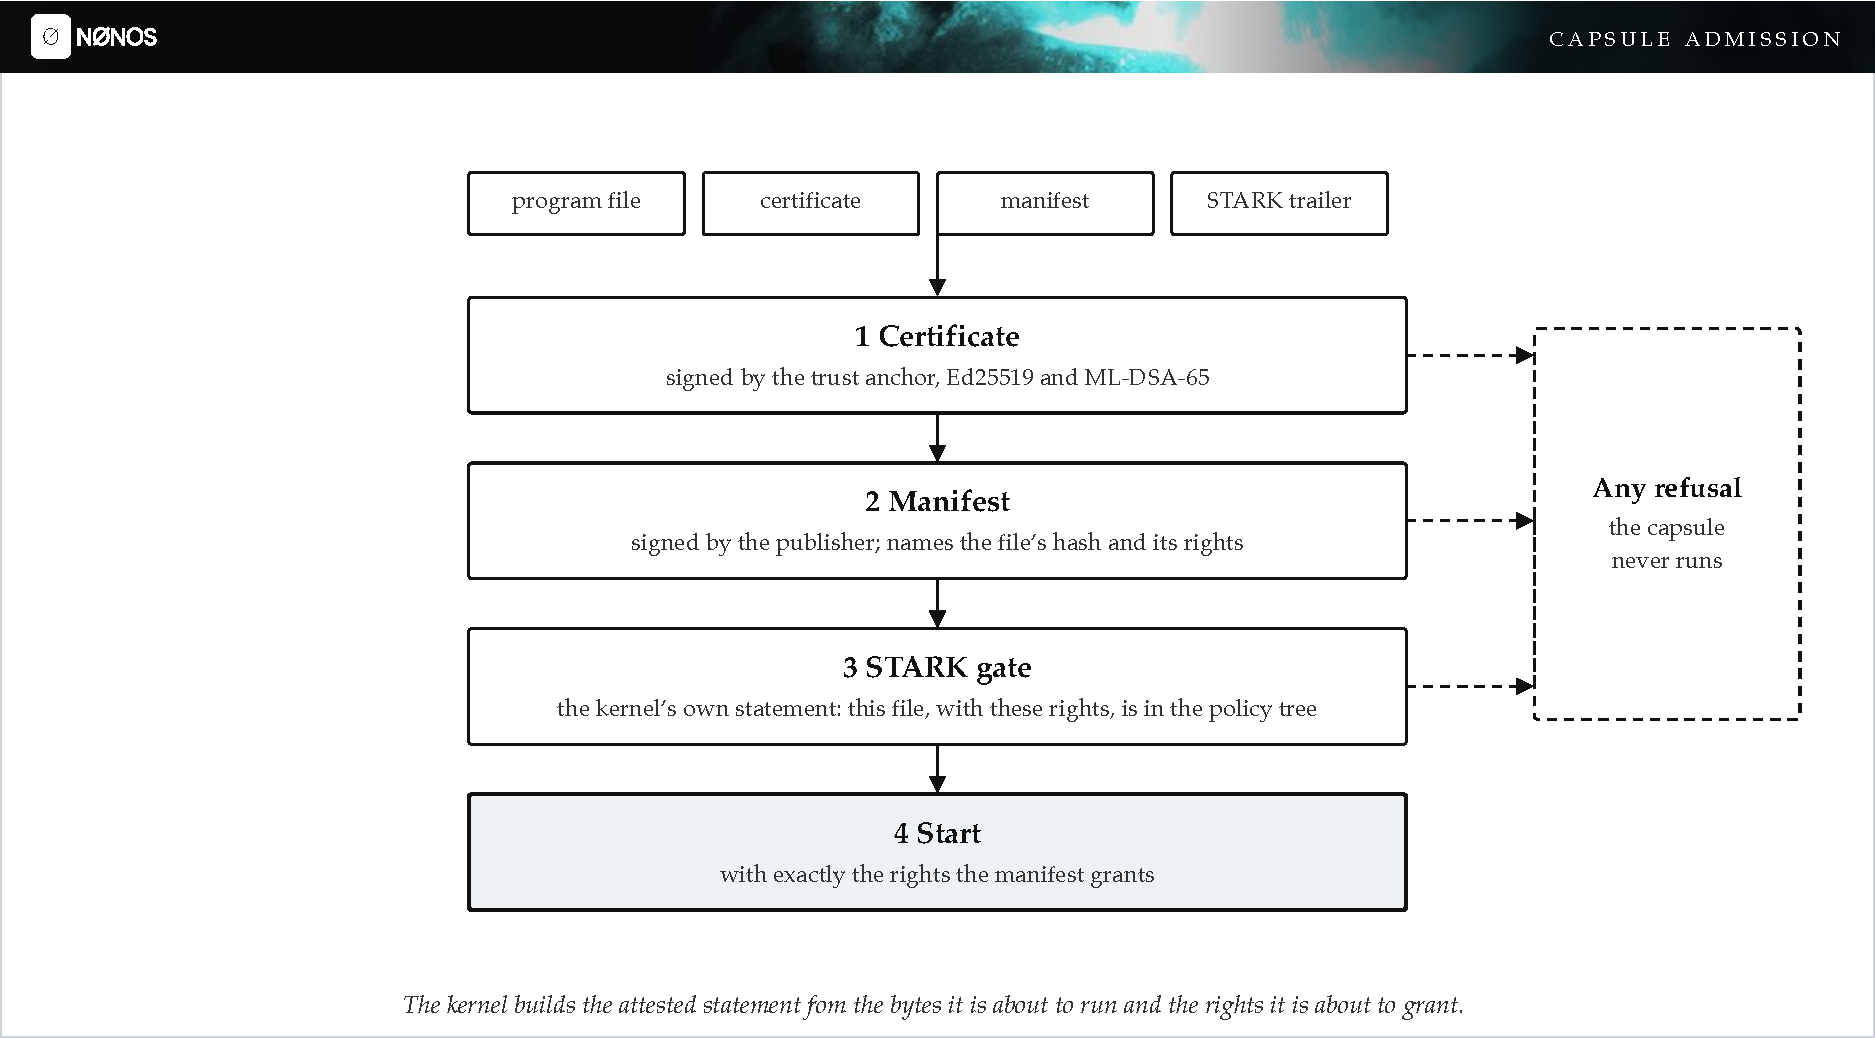
\includegraphics[width=0.84\textwidth]{figures/diagram-capsule-admission.pdf}
\caption{Capsule admission. The kernel builds the attested statement from the bytes it is about to run and the rights it is about to grant. Any refusal means the capsule never runs. Sources: \code{docs/security/boot-chain-and-signatures.md}, \code{docs/security/stark-attestation.md}.}
\label{fig:admit}
\end{figure}

A second admission path exists for code built on the machine itself. When the vendor root refuses a capsule, the kernel tries roots the person enrolled locally, and under such a root a trailer is a keyed tag the kernel minted for a local build instead of a STARK proof. The serial line \code{[ZK-ATTEST] ok} names the authority that admitted each capsule.\srcs{src/security/capsule_attest/against_root.rs:31-45}{docs/security/stark-attestation.md} The publisher tier, under which a capsule outside the project's namespace could run on its publisher's signature, admits no capsule in the release image.\src{docs/userland/signing-and-publisher-keys.md}

\subsection{An example: the Linux personality}

The capsule that matters most for this release is \code{capsule\_linux}, the Linux personality. Its \code{Capsule.mk} requires the word \code{0x104001979}: \code{CoreExec}, \code{IPC}, \code{Memory}, \code{Crypto}, \code{FileSystem}, \code{Debug}, two graphics bits, \code{StoreWrite} and \code{ForeignExec}. It lists \code{Network}, \code{LocalSign} and \code{StreamImport} as optional, with the word \code{0x600000004}.\src{userland/capsule_linux/Capsule.mk:50-59} The kernel holds a copy of the same list, and a comment there says the manifest is what the gate enforces.\src{src/userspace/capsule_linux/spawn.rs:36-55}

Two things about that word are worth stating, because Section~\ref{sec:box} depends on them. \code{ForeignExec} is the right to create a process the kernel has not verified, build its address space and answer its calls, and \code{capsule\_linux} is the only capsule in the tree whose \code{Capsule.mk} requests it.\src{docs/security/capsule-isolation-the-linux-personalitys.md} And \code{Network} is optional: it is held only by the instances that need it, which the personality's roles decide when they start, not by the program inside.\src{src/userspace/capsule_linux/roles.rs:32-58}

\subsection{Other capsules relevant to keys}

The keyring capsule holds the wallet's keys with no file, network or device access. It generates 12-word BIP-39 phrases, derives keys on \code{m/44'/60'/0'/0/i} for up to 8 accounts, and signs EIP-1559 transactions with in-process secp256k1, and it seals or opens the wallet's records only for a sender the service registry names as the wallet.\srcs{userland/capsule_keyring/src/server/hd.rs:37-60}{userland/capsule_keyring/src/server/vault_gate/mod.rs:17-25} The one caveat that matters is old: any capsule that holds both \code{Crypto} and \code{FileSystem} can ask the kernel for the vault root under its published label and read the sealed blob under \code{/data}, and the Linux personality, Settings and the Terminal are among those that hold both.\src{docs/security/protections-and-limits-what-nonos-does.md}
